\normaltrue \difficilefalse \tdifficilefalse
\correctionfalse

%\UPSTIidClasse{11} % 11 sup, 12 spé
%\newcommand{\UPSTIidClasse}{12}

\exer{Système bielle manivelle  $\star$ \label{B2:13:12}}
\setcounter{numques}{0}
\UPSTIcompetence[2]{B2-13}
\index{Compétence B2-13}
\index{Bielle Manivelle}
\index{Moteur}
\ifcorrection
\else
\textbf{Pas de corrigé pour cet exercice.}
\fi

\ifprof
\else
Soit le mécanisme suivant. On a $\vect{AB}=R\vect{i_1}$ et $\vect{CB}=L\vect{i_2}$. De plus, 
$R=\SI{10}{mm}$ et $L=\SI{20}{mm}$. 

\begin{center}
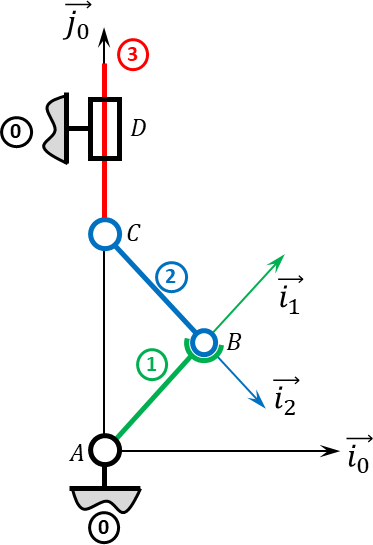
\includegraphics[width=\linewidth]{12_01}
\end{center}
\fi

Il est possible de mettre la loi entrée-sortie sous la forme  
$\lambda(t) = \pm\sqrt{L^2 - R^2\cos^2\theta(t)} + R\sin\theta(t) $ 
et 
$\lambdap(t) = \pm\left( \dfrac{R^2 \thetap(t) \cos\theta(t)\sin\theta(t)}{\sqrt{L^2 - R^2\cos^2\theta(t)}}\right) + \thetap(t)R\cos\theta(t)$.
 (à vérifier -- voir exercice \ref{C2:06:12}).

\question{Donner le torseur cinématique $\torseurcin{V}{2}{0}$ au point $B$.}
\ifprof
On commence par calculer $\vectv{B}{2}{0}$ = $\vectv{B}{2}{1}+\vectv{B}{1}{0}$ $=\vectv{B}{1}{0}$.
\begin{itemize}
\item \textbf{Méthode 1 -- dérivation vectorielle :}  $\vectv{B}{1}{0}$ $=\deriv{AB}{\rep{0}}$ 
$=\deriv{R\vi{1}}{\rep{0}}$ 
$= R\thetap(t) \vj{1}$. 
\item \textbf{Méthode 2 -- formule de changement de point: }
$\babarv{B}{A}{1}{0}$ 
$= -R\vi{1}\wedge \thetap{t} \vk{0}$
$= R\thetap(t) \vj{1}$.
\end{itemize}

On a alors, 
$\torseurcin{V}{2}{0}$
$=\torseurl{\varphip(t)\vk{0}}{R\thetap(t) \vj{1}}{B}$.

\else
\fi

\question{Donner le torseur cinématique $\torseurcin{V}{2}{0}$ et au point $C$.}

\ifprof
On a, 
$\torseurcin{V}{2}{0}$
$=\torseurl{\varphip(t)\vk{0}}{\lambdap(t) \vj{0}}{C}$.

Par ailleurs, on peut remarquer que 
$\babarv{C}{B}{2}{0}$
$= R\thetap(t) \vj{1} + L\vi{2}\wedge\varphip(t) \vk{0}$ 
$= R\thetap(t) \vj{1} - L\varphip(t)\vj{2}$.

On a donc nécessairement 
$\lambdap(t) \vj{0}= R\thetap(t) \vj{1} - L\varphip(t)\vj{2}$

$\Rightarrow \lambdap(t) \vj{0}= R\thetap(t) \left( \cos\theta(t)\vj{0}-\sin\theta(t)\vi{0} \right) - L\varphip(t)\left( \cos\varphi(t)\vj{0}-\sin\varphi(t)\vi{0}\right)$.

On a donc :

$
\left\{
\begin{array}{l}
0= -R\thetap(t) \sin\theta(t)  + L\varphip(t)\sin\varphi(t) \\
\lambdap(t) = R\thetap(t)  \cos\theta(t)- L\varphip(t)\cos\varphi(t)
\end{array}
\right.
$

$
\Rightarrow \left\{
\begin{array}{l}
R\thetap(t) \sin\theta(t)  = L\varphip(t)\sin\varphi(t) \\
\lambdap(t) - R\thetap(t)  \cos\theta(t)= L\varphip(t)\cos\varphi(t)
\end{array}
\right.
$

$\Rightarrow 
\tan \varphi(t) = \dfrac{R\thetap(t) \sin\theta(t) }{\lambdap(t) - R\thetap(t)  \cos\theta(t)}
$

Il resterait à supprimer $\varphi(t)$ pour (espérons-le) retomber sur la loi entrée-sortie cinématique.

\else
\fi


\question{Déterminer $\vectg{B}{2}{0}$.}
\ifprof
$\vectg{B}{2}{0}$
$=\deriv{\vectv{B}{2}{0}}{\rep{0}}$
$=\deriv{R\thetap(t) \vj{1}}{\rep{0}}$
$=R\thetapp(t) \vj{1} - R\thetap^2(t) \vi{1}$.
\else
\fi

\question{Déterminer $\vectg{C}{2}{0}$.}

\ifprof
$\vectg{C}{2}{0}$
$=\deriv{\vectv{C}{2}{0}}{\rep{0}}$
$=\lambdapp(t) \vj{0} $.
\else
\fi


\ifprof
\else
\begin{flushright}
\footnotesize{Corrigé  voir \ref{B2:13:12}.}
\end{flushright}%
\fi